% \subsection{Firma}
%     \vspace{0.5cm}
%     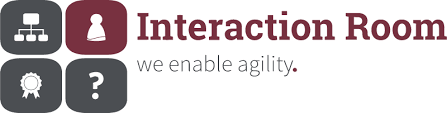
\includegraphics[width=0.6\textwidth]{images/IRG-Logo.png}
%     \vspace{0.5cm}
    
%     Die Interaction Room GmbH ist ein IT-Consulting-Dienstleister und Softwareentwicklungsunternehmen aus Essen, welches sich auf den Bereich agile Projektplanung konzentriert und dabei insbesondere den Umgang mit der sogenannten gezähmten Agilität vorantreibt. Im Rahmen eines universitären Forschungsprojekts ist die Methode Interaction Room entstanden, welche als Teil des Requirements-Engineerings zur Vorbereitung eines agil entwickelten Software-Projekts dient. Außerdem hat sie dem Unternehmen seinen Namen verliehen. Die Softwareentwicklung beinhaltet sowohl die Entwicklung intern genutzter Software als auch die Planung und Entwicklung externer Software-Projekte.

Kanban ist ein agiles Kommunikations-Framework, welches die Reaktionsfähigkeit und Effizienz eines Projektteams steigern soll. Dies wird durch einen Planungsprozess erreicht, der konstante neue Produktiterationen vorsieht und Arbeitsprozesse von Priorisierung und WIP-Limits abhängig macht.
Klassisch wird Kanban in agilen Softwareentwicklungsprojekten mit Entwicklungsteams von 8 bis 12 Teammitgliedern angewendet.
Die Flight-Level Methode beschränkt das Modell Kanban nicht mehr auf Projektteams, sondern sieht Anwendung in allen Unternehmensebenen, auch Flight-Level genannt, vor. Wird diese Methode erfolgreich auf allen Ebenen eingesetzt, erreicht die Organisation den sogenannten Status der Business-Agilität\cite{agilitaetNeuDenken}. 
Die Methode wurde von Klaus Leopold entwickelt und beinhaltet diese drei Flight-Level, die im Weiteren betrachtet werden\cite{agilesProjektmanagementImBerufsalltag}:

\begin{longtable}{p{3cm}p{10cm}}
    Flight-Level 1: & operative Ebene mit einem Projekt oder Team \cr
    Flight-Level 2: & Koordinierung der Zusammenarbeit mehrerer Teams\cr
    Flight-Level 3: & strategisches Portfoliomanagement
\end{longtable}